\documentclass[11pt, a4paper]{article}
\usepackage{graphicx}
\usepackage{amsmath}
\usepackage{listings}
\usepackage{alltt}
\usepackage{minted}
\usepackage{physics}
\usepackage{comment}

\title{\underline{\textit{\Large{Assignment 7: Analysis of Circuits using Laplace Transforms}}}}

\author{\textit{ROHIT KUMAR [EE20B111]}}

\date{\today} 

\begin{document}
\maketitle

\section*{Aim}
The goal of this assignment is the following:
\begin{itemize}
\item The analysis of filters using laplace transforms.
\item We look at an active low pass filter and an active high pass filter and to understand its nature.
\item Python’s  symbolic  solving  library,  sympy  is  a  tool  we  use  in  the  process  to handle our requirements in solving Modified Nodal Analysis equations. 

\end{itemize}

\section*{Low Pass Filter}
The low pass filter that we use gives the following matrix equation after simplification of the modified nodal equations.:-
\[\begin{pmatrix} 0 & 0 & 1 & -\frac{1}{G} \\ -\frac{1}{1+sR_2C_2} & 1 & 0 & 0 \\ 0 & -G & G & 1 \\ -\frac{1}{R_1}-\frac{1}{R_2}-sC_1 & \frac{1}{R_2} & 0 & sC_1 \end{pmatrix}\begin{pmatrix} V_1 \\ V_p \\ V_m \\ V_o \end{pmatrix} = \begin{pmatrix} 0 \\ 0 \\ 0 \\ -V_i(s)/R_1 \end{pmatrix}\]

The python code snippet that declares the low pass function and solves the matrix equation to get the V matrix is as shown below:
%\begin{minted}{python3}
\begin{verbatim}
def LowPass(R1, R2, C1, C2, G, Vi):
    	s = symbols('s')
    	A = Matrix([[0, 0, 1, -1/G],
    		[-1/(1 + s*R2*C2), 1, 0, 0],
    		[0, -G, G, 1],
    		[-1/R1-1/R2-s*C1, 1/R2, 0, s*C1]])
    	b = Matrix([0, 0, 0, -Vi/R1])
    	V = A.inv()*b
    	return A, b, V
\end{verbatim}
%\end{minted}
The plot for the magnitude of the transfer function (magnitude bode plot) is as shown below:
\begin{figure}[!tbh]
   	\centering
   	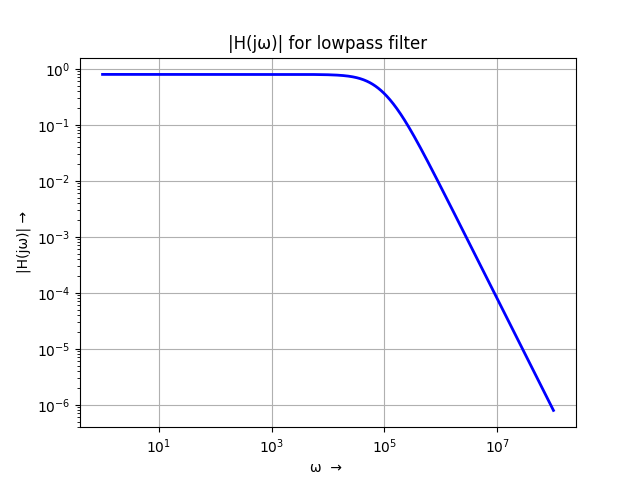
\includegraphics[width=1.0\textwidth]{Ass7_Figure_0.png}
   	\label{fig:32}
   	\caption{Low pass filter Magnitude response}
   \end{figure}

\section*{High Pass Filter}
The high pass filter we use gives the following matrix equations after simplification of the modified nodal equations
\[\begin{pmatrix} 0 & 0 & 1 & -\frac{1}{G} \\ -\frac{-sR_3C_2}{1+sR_3C_2} & 1 & 0 & 0 \\ 0 & -G & G & 1 \\ -1-(sR_1C_1)-(sR_3C_2)) & sC_2R_1 & 0 & 1 \end{pmatrix}\begin{pmatrix} V_1 \\ V_p \\ V_m \\ V_o \end{pmatrix} = \begin{pmatrix} 0 \\ 0 \\ 0 \\ -V_i(s)sR_1C_1 \end{pmatrix}\]

The python code snippet that declares the high pass function and solves the matrix equation to get the V matrix is as shown below:

%\begin{minted}{python3}
\begin{verbatim}
def HighPass(R1, R3, C1, C2, G, Vi):
    s = symbols("s")
	    A = Matrix([[0, -1, 0, 1/G],
        [s*C2*R3/(s*C2*R3+1), 0, -1, 0],
        [0, G, -G, 1],
        [-s*C2-1/R1-s*C1, 0, s*C2, 1/R1]])
    b = Matrix([0, 0, 0, -Vi*s*C1])
    V = A.inv()*b
    return A, b, V  
\end{verbatim}
%\end{minted}
The plot for the magnitude of the transfer function (magnitude bode plot) is as shown below:
\begin{figure}[!tbh]
   	\centering
   	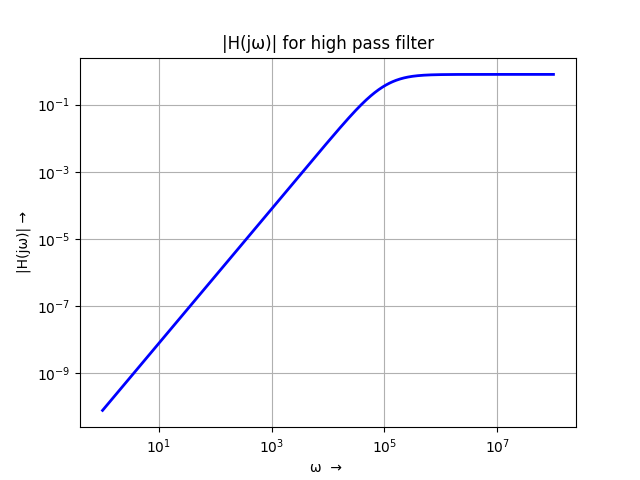
\includegraphics[width=1.0\textwidth]{Ass7_Figure_3.png}
   	\label{fig:32}
   	\caption{High pass filter Magnitude response}
   \end{figure}
\section*{Change of Format in Sympy Functions}
The sympy functions, that are expressed in terms of 's', must be converted to another form that is understood by sp.signal. This is done using the \textit{sympytoscipy()} function.\\
The python code snippet to do so is as shown:
%\begin{minted}{python3}
 \begin{verbatim}
def sympytoscipy(Y):
    	n, d = fraction(Y)
    	nr, dr = (np.array(Poly(n, s).all_coeffs(), dtype = float), np.array(Poly(d,
    	
    	s).all_coeffs(), dtype = float))
    	H = sp.lti(nr, dr)
    	return H
\end{verbatim}	
%\end{minted}

\section*{Step Response of Low Pass Filter}
In order to find the step response of the low pass filter, we need to assign $ Vi(s) = 1/s $. 
The python code below explains it. 
%\begin{minted}{python3}
\begin{verbatim}
    
A1, b1, V1 = LowPass(10000, 10000, 1e-9, 1e-9, 1.586, 1/s)
Vo1 = V1[3]
H1 = sympytoscipy(Vo1)
t, y1 = sp.impulse(H1, None, np.linspace(0, 5e-3, 10000))


# Plot for step response of a lowpass filter.
figure(1)
title("Step Response for low pass filter")
xlabel("t → ", fontsize = 13)
ylabel("v\u2092(t) → ", fontsize = 13)
plot(t, y1, 'b')
grid(True)
\end{verbatim}
%\end{minted}
The plot for the step response of the low pass circuit is as shown:
\begin{figure}[!tbh]
   	\centering
   	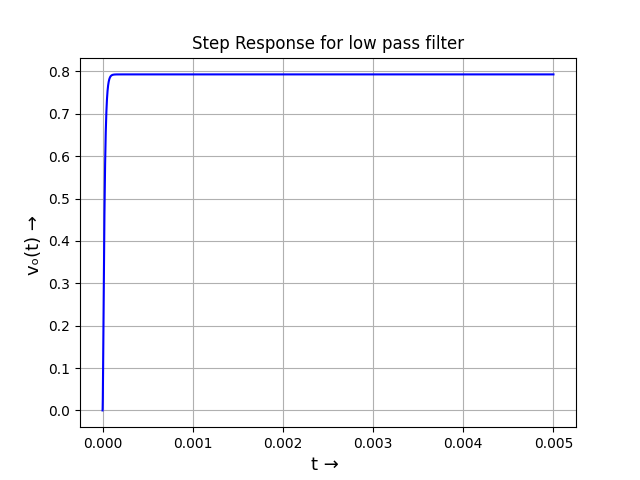
\includegraphics[width=1.0\textwidth]{Ass7_Figure_1.png}
   	\label{fig:32}
   	\caption{System Response of Low Pass Filter with Decay = 0.5.}
   \end{figure}
\section*{Response to the Sum Of Sinusoids}   
    When the input is a sum of sinusoids like,
\begin{equation*}
  V_{i}(t) = ( \ \cos(2*10^{6}\pi t) + sin(2000\pi t)\ )u_{o}(t) \ Volts
  \end{equation*}
  Then the output response for the lowpass filter can easily be found as shown in the code snippet.
%  \begin{minted}{python3}
\begin{verbatim}
    
s = symbols('s')
A, b, V = LowPass(10000, 10000, 1e-9, 1e-9, 1.586, 1)
Vo = V[3]
H = sympytoscipy(Vo)
ww = logspace(0, 8, 801)
ss = 1j*ww
hf = lambdify(s, Vo, 'numpy')
v = hf(ss)


vi = cos(2e6*pi*t) + sin(2000*pi*t) 
t, y2, svec = sp.lsim(H, vi, t)

figure(2)
plot(t, y2, 'b')
title("Output voltage for sum of sinusoids")
xlabel("t → ", fontsize = 13)
ylabel("v\u2092(t) → ", fontsize = 13)
grid(True)
\end{verbatim}
%  \end{minted}
The output response to the sum of sinusoids for the low pass filter is as shown:
\begin{figure}[!tbh]
   	\centering
   	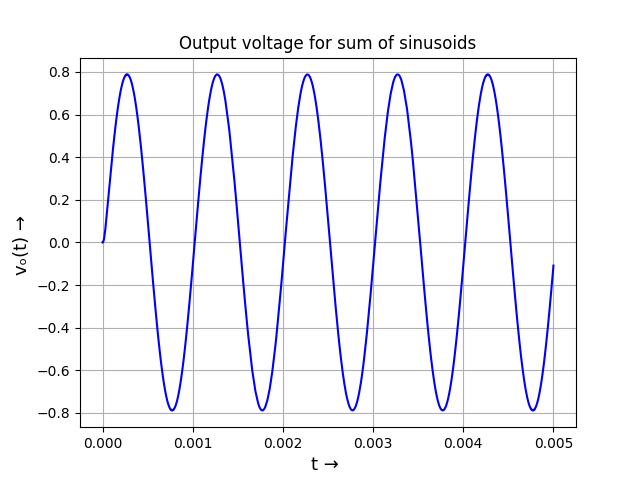
\includegraphics[width=1.0\textwidth]{Ass7_Figure_2.png}
   	\label{fig:32}
   	\caption{Output for sum of sinusoids}
   \end{figure}
   \newpage
\section*{Response to Damped Sinusoids}
In this case we assign the input voltage as a damped sinusoid like,\\
Low frequency,
\begin{equation*}
    V_{i}(t) = e^{-500t}( \ \cos(2000\pi t) \ )u_{o}(t) \ Volts
\end{equation*}
High frequency,
\begin{equation*}
    V_{i}(t) = e^{-500t}( \ \cos(2*10^{6}\pi t) \ )u_{o}(t) \ Volts
\end{equation*}
The high frequency and low frequency plots of the input damped sinusoids are as shown:\newpage
\begin{figure}[!tbh]
   	\centering
   	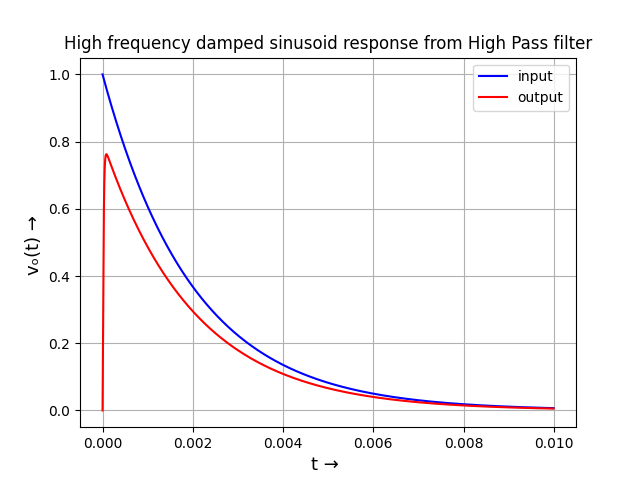
\includegraphics[width=1.0\textwidth]{Ass7_Figure_4.png}
   	\label{fig:32}
   	\caption{High frequency damped sinusoid}
   \end{figure}
\begin{figure}[!tbh]
   	\centering
   	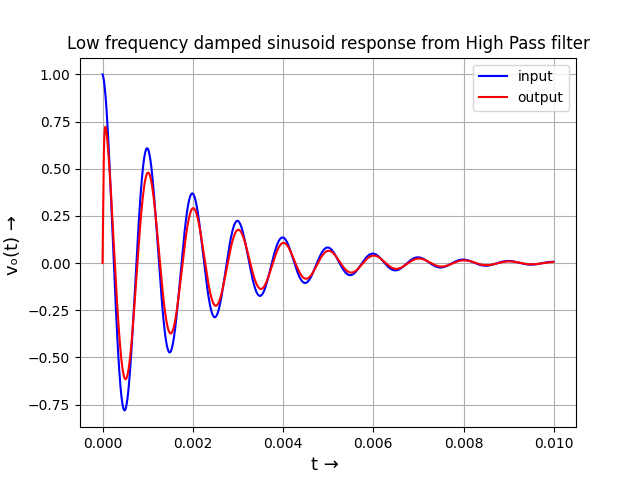
\includegraphics[width=1.0\textwidth]{Ass7_Figure_5.png}
   	\label{fig:32}
   	\caption{Low frequency damped sinusoid}
   \end{figure}
   
   Thus, the high-pass behaviour of the circuit is verified.  The change in the exponential would only affect the rate at which the sinusoid amplitude decays to zero.
The python code snippet to execute the above is as shown:
%\begin{minted}{python3}
\begin{verbatim}
    
A3, b3, V3 = HighPass(10000, 10000, 1e-9, 1e-9, 1.586, 1)
Vo3 = V3[3]
H3 = sympytoscipy(Vo)
hf3 = lambdify(s, Vo3, 'numpy')
v3 = hf3(ss)




t2 = arange(0, 1e-2, 1e-5) 
vi_d_1 = exp(-500*t2)*cos(2e6*pi*t2)
t2, y4, svec = sp.lsim(H3, vi_d_1, t2)


t3 = arange(0, 1e-2, 1e-5)    
vi_d_2 = exp(-500*t3)*cos(2e3*pi*t3)
t3, y4_2, svec = sp.lsim(H3, vi_d_2, t3)


figure(4)
plot(t2, vi_d_1, label = 'input', color = 'b')
plot(t2, y4, label = 'output', color = 'r')
title("High frequency damped sinusoid response from High Pass filter")
xlabel("t → ", fontsize = 13)
ylabel("v\u2092(t) → ", fontsize = 13)
grid(True)
legend()


figure(5)
plot(t3, vi_d_2, label = 'input', color = 'b')
plot(t3, y4_2, label = 'output', color = 'r')
title("Low frequency damped sinusoid response from High Pass filter")
xlabel("t → ", fontsize = 13)
ylabel("v\u2092(t) → ", fontsize = 13)
grid(True)
legend()
\end{verbatim}
%\end{minted}

%The output responses for both cases in a high pass filter is as shown:\newpage
%\begin{figure}[!tbh]
%   	\centering
%   	\includegraphics[scale=0.6]{Figure_7.png}
%   	\label{fig:32}
 %  	\caption{Output response of a high frequency damped sinusoid}
  % \end{figure}
%\begin{figure}[!tbh]
 %  	\centering
  % 	\includegraphics[scale=0.6]{Figure_8.png}
   %	\label{fig:32}
   	%\caption{Output response of a low frequency damped sinusoid}
   %\end{figure}

\section*{Step Response of High Pass Filter}
In order to find the step response of the high pass filter, we need to assign $ Vi(s) = 1/s $. 
The python code below shows:-
%\begin{minted}{python3}
\begin{verbatim}
    
A5, b5, V5 = HighPass(10000, 10000, 1e-9, 1e-9, 1.586, 1/s)
Vo5 = V5[3]
H5 = sympytoscipy(Vo5)
t5, y5 = sp.impulse(H5, None, linspace(0, 5e-3, 10000))


figure(6)
plot(t5, y5, 'b')
title("Step Response for high pass filter")
xlabel("t → ", fontsize = 13)
ylabel("v\u2092(t) → ", fontsize = 13)
grid(True) 
\end{verbatim}
%\end{minted}
The plot of the step response for a high pass filter is as shown:
\begin{figure}[!tbh]
   	\centering
   	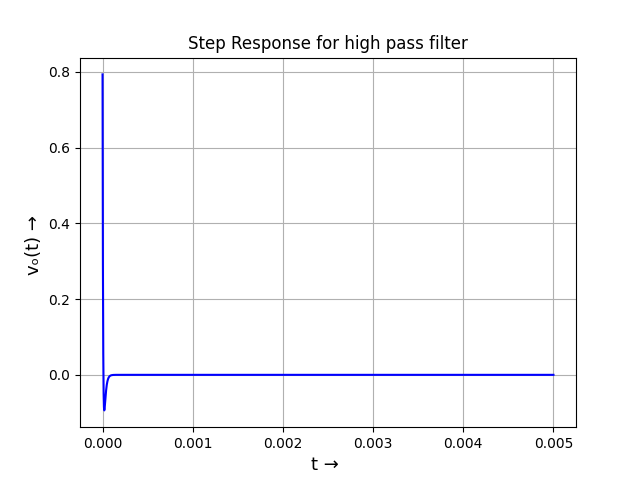
\includegraphics[width=1.0\textwidth]{Ass7_Figure_6.png}
   	\label{fig:32}
   	\caption{Step response for a high pass filter}
   \end{figure}\newpage
The unit step response, as expected is high at t=0 when there is an abrupt
change in the input. Since there is no other change at large time values outside
the neighbourhood of 0, the Fourier transform of the unit step has high values
near 0 frequency, which the high pass filter attenuates.

\section*{Conclusion}
\begin{itemize}
    \item  The low pass filter responds by letting the low frequency sinusoid pass through withoutmuch additional attenuation. The output decays as the input also decays.
    \item The high pass filter responds by quickly attenuating the input.  Notice that the time scalesshow  that  the  high  pass  filter  response  is  orders  of  magnitudes  faster  than  the  low  passresponse.  This is because the input frequency is below the cutoff frequency, so the outputgoes to 0 very fast.
    \item In conclusion, the sympy module has allowed us to analyse quite complicated circuits byanalytically solving their node equations. We then interpreted the solutions by plotting timedomain responses using the signals toolbox.  Thus, sympy combined with the scipy.signalmodule is a very useful toolbox for analyzing complicated systems like the active filters inthis assignment.
\end{itemize}  
\end{document}